\documentclass[dvipsnames]{beamer}
\usepackage{lmodern}
\usepackage{appendixnumberbeamer}
\renewcommand{\sfdefault}{lmss}
\renewcommand{\ttdefault}{lmtt}
\usepackage[T1]{fontenc}
% \usepackage[utf8]{inputenc}
\setcounter{secnumdepth}{3}
\setcounter{tocdepth}{3}
\usepackage{amsmath}
\usepackage{amsthm}
\usepackage{amssymb}
\theoremstyle{definition}
\newtheorem*{defn*}{\protect\definitionname}
\providecommand{\definitionname}{Definition}
\usepackage{graphicx}
\usepackage{hyperref}
\usepackage{ulem}
\PassOptionsToPackage{normalem}{ulem}
\usepackage{caption}
\usepackage{subcaption}
\usepackage{verbatim}
\usepackage[english]{babel}
\usepackage[autostyle]{csquotes}
\usepackage{tikz}
\usetikzlibrary{arrows,intersections}
\usepackage{pgfplots}
\pgfplotsset{compat = 1.15}
\usepgfplotslibrary{fillbetween}
\usepackage{verbatim}
\usepackage{booktabs}
\usepackage{multirow}
\usepackage{array}
\usepackage{nccmath}
% \usepackage{listings}
\usepackage{mathtools}

%Bibliography style, etc.
\usepackage[citestyle=authoryear-comp,natbib, uniquename = false, url = false, doi = false, uniquelist=false]{biblatex}
\renewbibmacro{in:}{}
\AtEveryBibitem{%
  \clearfield{volume}%
  \clearfield{number}
  \clearfield{month}
  \clearfield{issn}
  \clearfield{isbn}
  \clearfield{pages}
}

%\usepackage{cleveref}
\usepackage{setspace}
\makeatletter

% Macros
\providecommand{\tabularnewline}{\\}
\newcommand{\gr}{\textcolor{ForestGreen}} 
\newcommand{\rd}{\textcolor{red}}
\newcommand{\cb}{\textcolor{CornflowerBlue}} %this is the blue color you like; simply type \cb{X} where "X" is the color you want in blue
\newcommand{\vitem}{\vfill \item} %auto-centers items in lists
\newcommand{\fall}{\ \forall} %redefines "forall" (I don't like the default spacing)
\newcommand{\frall}{\quad \forall} %a \forall separated from the main math; this is the way it usually shows up in equations
\newcommand{\exist}{\ \exists} %same as \fall, but for \exists; they have the same ugly spacing
\newcommand{\R}{\mathbb{R}} %set of real numbers
\newcommand*\bigcdot{\mathpalette\bigcdot@{.5}} %different size for cdots
% \newcommand{\argmax}{\text{arg}\max}
\newenvironment{itemframe}
    {\frame{}\itemize}
    {\itemize\frame}
\newcommand\makebeamertitle{\frame{\maketitle}}%
\newtheoremstyle{named}{}{}{\itshape}{}{\bfseries}{.}{.5em}{\thmnote{#3's }#1}
\theoremstyle{named}
\newtheorem*{prop*}{Proposition}
% \newtheorem*{corollary}{Corollary}
\newtheorem*{namedtheorem}{Theorem} %allows named theorems
\newtheorem*{nameddef}{Definition}
\newtheorem{proposition}{Proposition}
\newtheorem*{assumption}{Assumption}
\newtheorem*{namedcorollary}{Corollary}
\newtheorem*{namedlemma}{Lemma}
\newtheorem*{axiom}{Axiom}
\newtheorem*{theorem*}{Theorem}
\newtheorem*{lemma*}{Lemma}
\DeclareMathOperator*{\argmin}{argmin}
\DeclareMathOperator{\argmax}{argmax}
\DeclareMathOperator{\supp}{supp}
\DeclareMathOperator{\interior}{int}
\DeclareMathOperator{\rank}{rank}
\newcolumntype{C}[1]{>{\centering\let\newline\\\arraybackslash\hspace{0pt}}m{#1}}
\newcommand{\sbt}{\,\begin{picture}(-1,1)(-1,-3)\circle*{2}\end{picture}\ }



%formatting
\usetheme{Ilmenau}
\definecolor{MIT}{rgb}{.639,.122,.204}
\definecolor{UCLA}{rgb}{0.15294117647058825, 0.4549019607843137, 0.6823529411764706}
\definecolor{UCLA_gold}{rgb}{1, 0.8196078431372549, 0}
\usecolortheme[named=UCLA]{structure}
\setbeamercolor*{palette secondary}{fg=UCLA_gold,bg=gray!15!white}
\usecolortheme{dolphin}
\setbeamertemplate{navigation symbols}{} 
\setbeamertemplate{footline}{}{}
\setbeamertemplate{headline}{}
\setbeamertemplate{navigation symbols}{}
\mode<presentation> {}
\setbeamercolor{block title}{use=structure,fg=white,bg=RoyalBlue} %blocks (theorems, etc.)in blue
\setbeamercolor{block title alerted}{use=structure,fg=white,bg=ForestGreen} %blocks (theorems, etc.)in blue

\renewcommand\qedsymbol{$\blacksquare$} %set QED symbol as black square
\renewcommand{\emph}{\textit} %set emphasized text style; this is italics
\setbeamertemplate{footline}[frame number] %slide numbers
\setbeamertemplate{itemize item}[circle] %bullet style
\setbeamertemplate{itemize subitem}{--}
\setbeamertemplate{enumerate item}[default]
\newrobustcmd*{\parentexttrack}[1]{%
  \begingroup
  \blx@blxinit
  \blx@setsfcodes
  \blx@bibopenparen#1\blx@bibcloseparen
  \endgroup}

\AtEveryCite{%
  \let\parentext=\parentexttrack%
  \let\bibopenparen=\bibopenbracket%
  \let\bibcloseparen=\bibclosebracket}

 \AtBeginDocument{%
   \let\origtableofcontents=\tableofcontents
   \def\tableofcontents{\@ifnextchar[{\origtableofcontents}{\gobbletableofcontents}}
   \def\gobbletableofcontents#1{\origtableofcontents}
 }
\newcommand{\backupbegin}{
   \newcounter{framenumberappendix}
   \setcounter{framenumberappendix}{\value{framenumber}}
}
\newcommand{\backupend}{
   \addtocounter{framenumberappendix}{-\value{framenumber}}
   \addtocounter{framenumber}{\value{framenumberappendix}} 
} 

\renewcommand{\maketitle}{
\setbeamertemplate{footline}{} 
\begin{frame}[noframenumbering]
\titlepage
\end{frame}
\setbeamertemplate{footline}[frame number]
}

\usefonttheme[onlymath]{serif}

% \usetheme{CambridgeUS}

% \newtheorem{theorem}{Theorem}
% \theoremstyle{claim}
\newtheorem{claim}{Claim}
% \newtheorem{corollary}{Corollary}


\makeatother


%\author{Drew Fudenberg}

\institute[]{}
\title{Learning and Forgetting: The Dynamics of Aircraft Production}
\author{C. Lanier Benkard}

\begin{document}
\maketitle
\begin{frame}{Overview}
  \begin{itemize}
  \item Well-documented process of learning in organizations as they increase production over time.
    \vitem But do organizations also \emph{forget} over time?
    \vitem Benkard looks at detailed data on aircraft production at Lockheed from 1970--1984, and estimates a variety of production functions to see which one fits best.
    \begin{itemize}
    \item Also looks at imperfect spillovers across models.
    \end{itemize}
  \end{itemize}
  \begin{definition}[Organizational Forgetting]
   The hypothesis that the firm's production experience depreciates over time. 
  \end{definition}
\end{frame}
%
\begin{frame}{Data (Motivation)}
  \begin{figure}[htp]
    \centering
    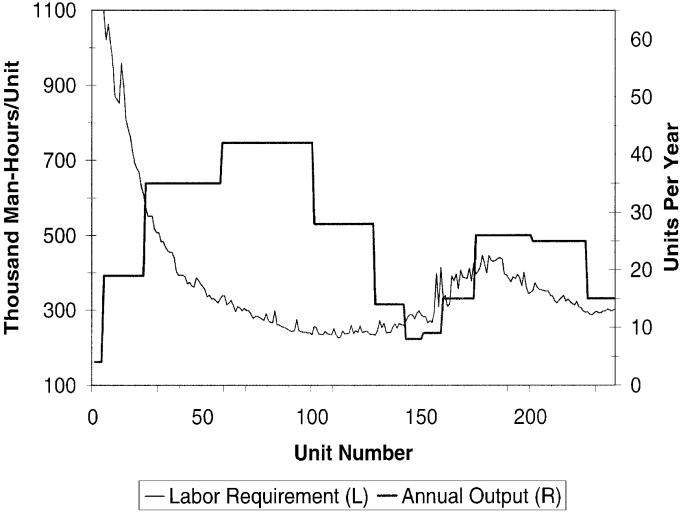
\includegraphics[width=\textwidth, keepaspectratio=true]{fig1.jpg}
  \end{figure}
\end{frame}
%
\begin{frame}{Industry Overview}
  \begin{itemize}
  \item Unlike military contracts, highly volatile demand/output for commercial planes.
    \vitem Reasonable amounts of competition; firms compete for customers by offering customizable options (in this case another model type). 
    \vitem Labor heavily unionized, and seniority structure leads to very high turnover (extra scope for retraining and forgetting).
  \end{itemize}
\end{frame}
%
\begin{frame}{Model of Production}
  \vspace{-2em}
  \begin{align*}
    q &= \min (G(L, E, \overline{K}, S, \varepsilon),
        H(M, E, \overline{K}, S, \nu )) \tag{Leontief} 
  \end{align*}
  \vspace{-1em}
  \begin{itemize}
  \item $E$ is experience (the main focus in the paper)
    \vitem $S$ is line speed (endogenous)
    \vitem $\varepsilon$ is a productivity shock to labor
    \vitem $\nu$ is a productivity shock to materials
  \end{itemize}
  \vfill
  Recall that unit production is very low, so $E$ changes meaningfully for each unit, and it's not crazy to think firms are adjusting variable inputs for each unit.
\end{frame}
%
\begin{frame}{Experience}
\begin{fleqn}[0pt]
  \begin{align*}
    E_i &= E_{i - 1} + 1; \quad E_{1} = 1 \tag{baseline}\\[2em]
    E_i &= \delta E_{i - 1} + q_{t - 1} \tag{with forgetting}\\[2em]
    E_i &= \left\{
          \begin{array}{lcl}
            E_{1, t}& : & i \in \{-1, -100, -200\}\\
            E_{500, t} & : & i = -500
          \end{array}\right. \tag{inc. spillovers}\\[1em]
    E_{1, t} &= \delta E_{1, t - 1} + q_{1, t - 1} + \lambda q_{500, t - 1}\\
    E_{500, t} &= \delta E_{500, t - 1} + \lambda q_{1, t - 1}
  \end{align*}
  \end{fleqn}
  \begin{itemize}
  \item $\lambda$ is the experience spillover parameter
    \vitem $\delta = 1$ and $\lambda =1$ recovers the baseline case
  \end{itemize}
\end{frame}
%
\begin{frame}{Estimation}
  \begin{itemize}
  \item Estimation via GMM; need instruments for line speed and experience
   \vitem Line speed should be correlated with current output; experience should be correlation with recent output 
   \vitem Benkard uses current and lagged demand and cost shifters
   \vitem \textbf{Demand Shifters:} Various world GDP measures, oil price, time trend
   \vitem \textbf{Cost Shifters:} World aluminum price and U.S. manufacturing wage
  \end{itemize}
\end{frame}
%
\begin{frame}{Results (no forgetting)}
  \begin{figure}[htp]
    \centering
    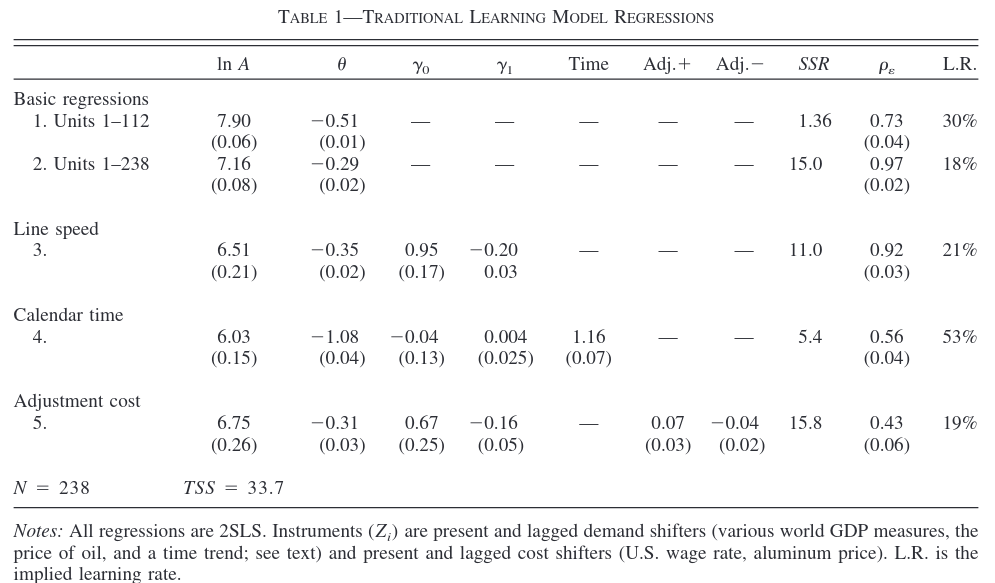
\includegraphics[width=\textwidth, keepaspectratio=true]{table1.png}
  \end{figure}
\end{frame}
%
\begin{frame}{Results (no forgetting)}
  \begin{figure}[htp]
    \centering
    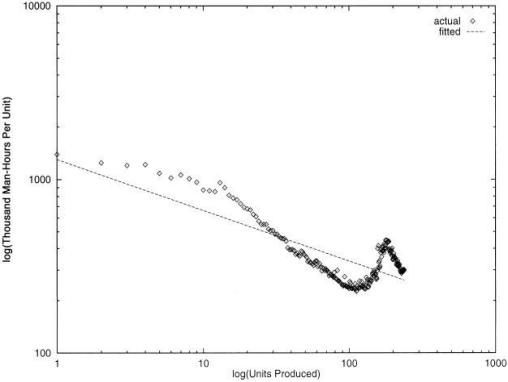
\includegraphics[width=\textwidth, keepaspectratio=true]{fig3.jpg}
  \end{figure}
\end{frame}
%
\begin{frame}{Testing the Production Function}
  \begin{figure}[htp]
    \centering
    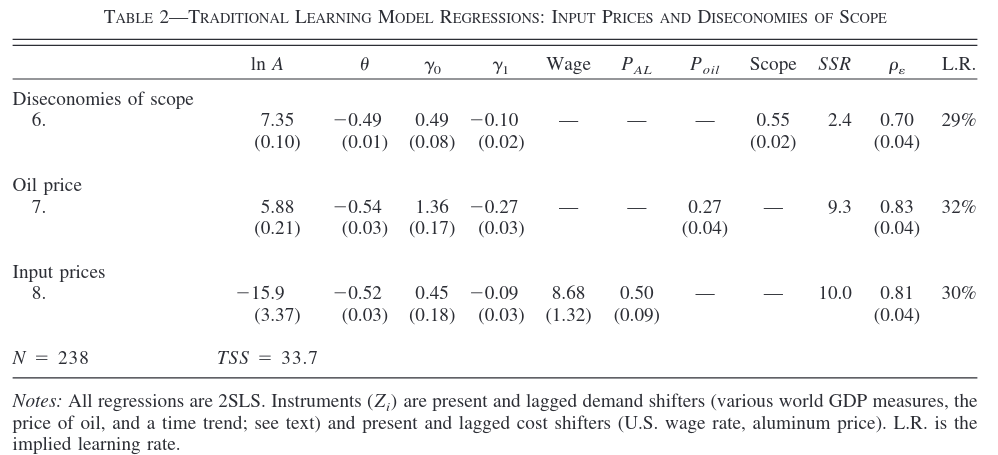
\includegraphics[width=\textwidth, keepaspectratio=true]{table2.png}
  \end{figure}
  \begin{itemize}
  \item (6) tests diseconomies of scope (plausible)
    \vitem (7--8) test for Cobb-Douglas (sign on wage is wrong)
    \vitem Can we do better than just a scope dummy?
  \end{itemize}
\end{frame}
%
\begin{frame}{Fitting the General Learning Model}
  \begin{figure}[htp]
    \centering
    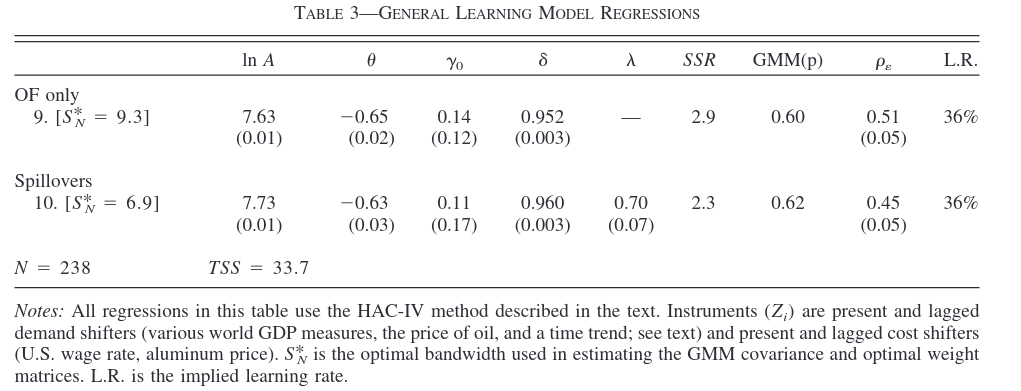
\includegraphics[width=\textwidth, keepaspectratio=true]{table3.png}
  \end{figure}
  \begin{itemize}
  \item Adding deprection causes SSR to fall $12.9 \to 2.9$, and $\delta \ne 1$
    \vitem Adding the spillover parameter $\lambda$ increases $\delta$
    \begin{itemize}
    \item This accounts for some of the confounding effects of the introduction of the $-500$ series
    \end{itemize}
  \end{itemize}
\end{frame}
%
\begin{frame}{Fitting the General Learning Model}
  \begin{figure}[htp]
    \centering
    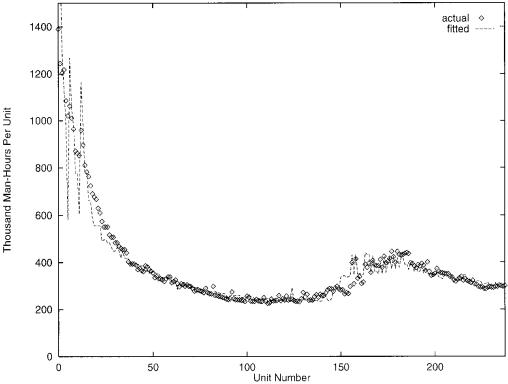
\includegraphics[width=\textwidth, keepaspectratio=true]{fig4.jpg}
  \end{figure}
\end{frame}
%
\begin{frame}{General Learning Model}
  \begin{itemize}
  \item Fits both halves of the data
    \vitem Outperforms the diseconomies of scope model from unit 140 onwards
    \begin{itemize}
    \item Captures $-500$ production becoming less efficient, and the increasing labor requirements for $-1$ planes
    \end{itemize}
    \vitem Implied depreciation rate $\delta = 0.96$ means that a firm ``forgets'' 39\% of its knowledge in a year
    \begin{itemize}
    \item Note that the definition of forgetting is \emph{very} specific---it's only looking at a narrow type of human capital
    \end{itemize}
    \vitem Allowing for depreciation increases the learning rate to 35\%--40\%
    \vitem $\lambda$ is always significant and never equal to 1; reject perfect spillovers
  \end{itemize}
\end{frame}
%
\begin{frame}{Results}
 Take $\lambda = 0.70$ and $\theta = 0.63$ 
 \begin{itemize}
 \item The first $-500$ required 25\% more labor than a $-1$
   \vitem Producing both $-500$s and $-1$s in similar numbers would have increased labor requirements by 11\%
   \vitem Introducing a similar model can cause a setback in learning and an increase in variable costs
   \vitem Simultaneous production of multiple models can be meaningfully more expensive (without accounting for R\&D)
 \end{itemize}
\end{frame}
%
\begin{frame}{Takeaways}
  \begin{itemize}
  \item Production dynamics in the airplane manufacturing industry are \emph{not} smooth; they're actually pretty complex.
    \vitem So far, we have only seen forgetting in industries that produce labor intensive products, with a lot of learning at the individual level, and high turnover.
    \begin{itemize}
    \item Aircraft manufacturing, ship building, service franchises
      \item Don't blindly start using this model everywhere
    \end{itemize}
    \vitem \textbf{Stochastic interpretation:} estimating a stochastic learning model yields very similar results
    \begin{itemize}
    \item Can think of learning as stochastic at the individual task level
      \item Unit-level data, while still pretty granular, aggregates over this uncertainty so the model is approximately deterministic
    \end{itemize}
  \end{itemize}
\end{frame}
\end{document}
%%% Local Variables:
%%% mode: latex
%%% TeX-master: t
%%% End:
